% This is "sig-alternate.tex" V2.0 May 2012
% This file should be compiled with V2.5 of "sig-alternate.cls" May 2012
%
% This example file demonstrates the use of the 'sig-alternate.cls'
% V2.5 LaTeX2e document class file. It is for those submitting
% articles to ACM Conference Proceedings WHO DO NOT WISH TO
% STRICTLY ADHERE TO THE SIGS (PUBS-BOARD-ENDORSED) STYLE.
% The 'sig-alternate.cls' file will produce a similar-looking,
% albeit, 'tighter' paper resulting in, invariably, fewer pages.
%
% ----------------------------------------------------------------------------------------------------------------
% This .tex file (and associated .cls V2.5) produces:
%       1) The Permission Statement
%       2) The Conference (location) Info information
%       3) The Copyright Line with ACM data
%       4) NO page numbers
%
% as against the acm_proc_article-sp.cls file which
% DOES NOT produce 1) thru' 3) above.
%
% Using 'sig-alternate.cls' you have control, however, from within
% the source .tex file, over both the CopyrightYear
% (defaulted to 200X) and the ACM Copyright Data
% (defaulted to X-XXXXX-XX-X/XX/XX).
% e.g.
% \CopyrightYear{2007} will cause 2007 to appear in the copyright line.
% \crdata{0-12345-67-8/90/12} will cause 0-12345-67-8/90/12 to appear in the copyright line.
%
% ---------------------------------------------------------------------------------------------------------------
% This .tex source is an example which *does* use
% the .bib file (from which the .bbl file % is produced).
% REMEMBER HOWEVER: After having produced the .bbl file,
% and prior to final submission, you *NEED* to 'insert'
% your .bbl file into your source .tex file so as to provide
% ONE 'self-contained' source file.
%
% ================= IF YOU HAVE QUESTIONS =======================
% Questions regarding the SIGS styles, SIGS policies and
% procedures, Conferences etc. should be sent to
% Adrienne Griscti (griscti@acm.org)
%
% Technical questions _only_ to
% Gerald Murray (murray@hq.acm.org)
% ===============================================================
%
% For tracking purposes - this is V2.0 - May 2012

\documentclass{sig-alternate}

\begin{document}
%
% --- Author Metadata here ---
\conferenceinfo{DEBS}{2014, India}
%\CopyrightYear{2007} % Allows default copyright year (20XX) to be over-ridden - IF NEED BE.
%\crdata{0-12345-67-8/90/01}  % Allows default copyright data (0-89791-88-6/97/05) to be over-ridden - IF NEED BE.
% --- End of Author Metadata ---

\title{Predicting Power Needs in Smart Grids - DEBS 2014 Grand Challenge}
%\titlenote{A full version of this paper is available as
%\textit{Author's Guide to Preparing ACM SIG Proceedings Using
%\LaTeX$2_\epsilon$\ and BibTeX} at
%\texttt{www.acm.org/eaddress.htm}}}
%
% You need the command \numberofauthors to handle the 'placement
% and alignment' of the authors beneath the title.
%
% For aesthetic reasons, we recommend 'three authors at a time'
% i.e. three 'name/affiliation blocks' be placed beneath the title.
%
% NOTE: You are NOT restricted in how many 'rows' of
% "name/affiliations" may appear. We just ask that you restrict
% the number of 'columns' to three.
%
% Because of the available 'opening page real-estate'
% we ask you to refrain from putting more than six authors
% (two rows with three columns) beneath the article title.
% More than six makes the first-page appear very cluttered indeed.
%
% Use the \alignauthor commands to handle the names
% and affiliations for an 'aesthetic maximum' of six authors.
% Add names, affiliations, addresses for
% the seventh etc. author(s) as the argument for the
% \additionalauthors command.
% These 'additional authors' will be output/set for you
% without further effort on your part as the last section in
% the body of your article BEFORE References or any Appendices.

\numberofauthors{4} %  in this sample file, there are a *total*
% of EIGHT authors. SIX appear on the 'first-page' (for formatting
% reasons) and the remaining two appear in the \additionalauthors section.
%
\author{
% You can go ahead and credit any number of authors here,
% e.g. one 'row of three' or two rows (consisting of one row of three
% and a second row of one, two or three).
%
% The command \alignauthor (no curly braces needed) should
% precede each author name, affiliation/snail-mail address and
% e-mail address. Additionally, tag each line of
% affiliation/address with \affaddr, and tag the
% e-mail address with \email.
%
Aman Mangal,~Arun Mathew,~Tanmay Randhavane,~Umesh Bellur
  \\ \affaddr{Department of Computer Science and
    Engineering}\\ \affaddr{Indian Institute of Technology-
    Bombay, Powai,  Mumbai-400076}\\ \email{\{amanmangal,~arunmathew,~tanmayr,~umesh\}@cse.iitb.ac.in}
% 2nd. author
}

% There's nothing stopping you putting the seventh, eighth, etc.
% author on the opening page (as the 'third row') but we ask,
% for aesthetic reasons that you place these 'additional authors'
% in the \additional authors block, viz.
%\additionalauthors{Additional authors: John Smith (The Th{\o}rv{\"a}ld Group,
%email: {\texttt{jsmith@affiliation.org}}) and Julius P.~Kumquat
%(The Kumquat Consortium, email: {\texttt{jpkumquat@consortium.net}}).}
%\date{30 July 1999}
% Just remember to make sure that the TOTAL number of authors
% is the number that will appear on the first page PLUS the
% number that will appear in the \additionalauthors section.

\maketitle
\begin{abstract}
Smart grids are becoming ubiquitous today with proliferation of easy to install power generation schemes for Solar and Wind energy. The attempt to consume energy locally generated instead of transmitting it over large distances calls for systems that can process millions of events being generated from smart plugs and power generation sources in near real time. The heart of these systems often is a module that can process dense power consumption event streams and predict the consumption patterns at specific occupational units such as a house or a building. It is also often useful to identify outliers that are consuming power significantly higher than other similar devices in the occupational unit (such as a block or a neighborhood). In this paper, we present a system that can process several million events per minute from smart plugs and correlate the information to output both predictions as well as identify outliers.
\end{abstract}

% A category with the (minimum) three required fields
%\category{H.4}{Information Systems Applications}{Miscellaneous}
%A category including the fourth, optional field follows...
%\category{D.2.8}{Software Engineering}{Metrics}[complexity measures, performance measures]

%\terms{Theory}

\keywords{smart grids, event processing}

\section{Introduction}
%This file will contain the introduction
%A little bit of the background of the problem goes here. %Query 1 and 2 are explained briefly.

The paper is structured as follows: In section 2, we detail our design approach. Section 3, 4 describes the system architecture and experimental results for Query 1,2 respectively. We present some of the ideas, which we could not implement as part of the current solution, in section 5 as future work. We conclude the paper in section 6.


\section{Design Approach}
%This file will contain our design approach
%Describe the basis and then the architecture here - for example how do you calculate medians, what kind of parallelism model is employed? How often do you need to synchronize? etc.
\subsection{Query 1}
In the context of query 1, time is divided into multiple slots of different time slice sizes. The time slice sizes considered are 1m, 5m, 15m, 60m \& 120m. Hence for a day we have twelve 120m slices and 86400 one minute slices. When processing the events falling withing a time slice, Query 1 should output predicted load of each plug and the house for the next to next time slice. Query 1 should output the load prediction based on the average load of current time slice and the median of the historical load averages of the future time slice for which we are making prediction. We need to produce forecast every 30s.

We have one house process for each house in the data set and a broker process. The broker process reads the data from the input stream (sorted events file in current implementation) and passes it to the corresponding house process. Communication between the processes is done via operating system sockets.

In the house process, we have load value accumulators for different time slices (1m, 5m, 15m, 60m and 120m). We also have another accumulator for 30s. When house process gets an event if the event falls within the current 30s time slice, the load \footnote{For now we are ignoring events with work values} value is added to the 30s accumulator and the count of values is incremented. If the event crosses the 30s timeslice, then the accumulated load values and count is added to accumulators of all the other time slices (1m, 5m $\cdot$ etc) and a forecast output is triggered, before setting the 30s accumulator to current load value and count to 1. The triggered forecasting will output the predictions for all the time slices with the average of current accumulated load values and the historical median of the corresponding future time slice. The accumulators for each time slice gets reset, if we get an event crossing the time slice boundary, after making the forecast using the accumulater load value.


\subsubsection{The Median Algorithm for query 1}
For this query, to forecast the load of a plug in a time slice of a specific size, we need the median of the previous average loads for that time slice and for that slice size. For each day and each plug, we have only one value per day of data for that time slice and slice size. So, we store all these values in a container.

In the median container we maintain two heaps. Out of the two, one is a min-heap and the other is a max-heap. Each heap contains about half of the values. Now following three cases can occur:
\begin{itemize}
\item Case 1: The min-heap contains one more element than the max-heap. In this case, the median is the topmost value of min-heap.
\item Case 2: The max-heap contains one more element than the min-heap. In this case, the median is the topmost value of max-heap.
\item Case 3: Both the min-heap and the max-heap contain equal number of elements. In this case, the median is the average of the topmost value of min-heap and the topmost value of max-heap.

\end{itemize}

\section{Query 2}
The goal of query 2 is to identify outliers that consume significantly higher amount of energy compared with the average consumption computed globally. A plug is counted as an outlier if median load of the plug is more than the median load of all the plugs in the system for a given sliding window (1 hr or 24 hrs). We need to produce an output event when the percentage of such plugs in a house changes from the previous position of the sliding window. 

\subsection{Architecture}
To evaluate Query 2, we have to compute global median i.e. median of all the data of all the plugs in the system acquired in a given sliding window of length 1 hr and 24 hrs. We compare the global median with the local plug medians and figure out the outliers in the system. All of this computation needs to be done every time we receive a new event. The frequent comparison of locally computed data with global data enforces a single node solution for all the houses in case of Query 2.

There are two processes in the system residing on different nodes. The broker process reads data from a file and sends events to the Q2 process. Q2 keeps a linked list of all the events of last 24 hrs in the order they have been received. Whenever a new event is received by Q2, we slide the window such that some of the events from the tail of the linked list are removed and the new event is inserted at the head. Further, required plug medians and global median are recomputed and change in the number of outlier plugs is written to the output file (denoting an output event).

\begin{figure}[h]
\begin{center}
\begin{tikzpicture}[scale=0.7, >=stealth', transform shape, shorten >=1pt, node distance=4cm,auto]
\tikzstyle{every state}=[draw=blue!50, very thick, fill=blue!20,minimum size=2cm]
\node[state] (broker) [text width=1.5cm, align=center] {Broker Process};
\node[state] (Q2) [right of=broker] {Q2 Process};

\path[->] (broker) edge node {events} (Q2);
\end{tikzpicture}
\caption{System Architecture (Query 2)}
\end{center}
\end{figure}
\vspace*{-0.3cm}

We use the Sliding Median Container (SlidingMc) in order to compute various medians and S Container (SCont) for the purpose of finding the number of outliers in every house. Let's assume an event \textit{E} is received by the Q2 process from the broker process with timestamp \textit{$T_E$}. Let's also assume the window size to be \textit{W} seconds which can be either 1 hr or 24 hrs. \textit{$T_W$} is the minimum timestamp which exists in the window of length \textit{W} terminating with the event E as shown in the Figure \ref{fig:linked_list}.

\begin{figure}[h]
\begin{center}
\begin{tikzpicture}[scale=0.8, transform shape, shorten >=1pt, node distance=0.8cm,auto]
\tikzstyle{every state}=[draw=blue!50, rectangle, very thick, fill=blue!20]
\node[state] (I1) {$T_0$};
\node[state] (I2) [right of=I1] {};
\node[state] (I3) [right of=I2] {};
\node[state] (I4) [right of=I3] {$$};
\node[state] (I5) [right of=I4] {$T_W$};
\node[state] (I6) [right of=I5] {$$};
\node[state] (I7) [right of=I6] {$$};
\node[state] (I8) [right of=I7] {$$};
\node[state] (I9) [right of=I8] {$T_E$};

\draw [decorate,decoration={brace,amplitude=10pt,mirror,raise=10pt},yshift=0pt] (I5.center) -- (I9.center);
\node (text) at (5,-1) {Window W};
\end{tikzpicture}
\caption{Linked List in Q2 process \label{fig:linked_list}}
\end{center}
\end{figure}

Note that there may be multiple events with the timestamp $T_W$ in the window. In such a case, we choose the left most event with the same timestamp $T_W$ in the linked list. Also, if the data corresponding to the timestamp $\tau = (T_E - W +1)$ is missing, then $T_W$ will be the first timestamp bigger than $\tau$ for which event for any plug in the system is present. Now, the algorithm proceeds as follows. We shift the left end of the window one event, keeping the right end fixed. We delete the oldest event from the median container of the corresponding plug and the global median container. Now, we compute new median of the plug and insert the new median into the S container of the house. S container is, then, queried to find out whether the percentage of outliers for a given house has changed after the shift. We output an event if any of the percentage for any house has changed. On the other hand, if the global median doesn't change, we only check the percentage number of outliers for the house corresponding to the deleted event.

We stop when the leftmost event in the window has the timestamp $T_W$. In the last slide, before computing any medians, we also insert the newly received event $E$ into the global median container and the median container of the plug of the event E. Rest of the computation remains same. To avoid redundant storage of the data, we keep the linked list only for 24 hrs sliding window, and keep a pointer to the first event of the 1 hr window in the same linked list.


\subsection{Median Algorithm}
In query 2, we have to compute the median of large amounts of data frequently. A trade off exists between the computational complexity and accuracy of the median so derived. We define a container which provides the basic functionality of inserting a new element, deleting a given element and finally providing the approximate median for currently existing data in the container. We first insert all the elements into the container corresponding to the sliding window. Every time we slide by 1 sec, we perform at most 2 operations. We delete the oldest event if it exists and insert the latest event in the window. Every insert and/or delete operation is followed by computation of median. We, therefore, want to minimize the complexity of median calculation. We, now, propose an algorithm to compute median which takes constant time for every operation in the given scenario with very low relative error.

The basic idea is to construct a histogram of the data using fixed number of bins (M-1)\footnote{The Algorithm is inspired from discussions on \url{http://stackoverflow.com/questions/638030}} . The histogram is then queried to find median of the data. We sort the first M distinct values inserted into the container and use them in order to build up the (M-1) bins. Every $i^{th}$ inserted value corresponds to the starting of $i^{th}$ bin and every bin is associated with a frequency. Frequency denotes the frequency of the data greater than equal to $i^{th}$ lowest value (including) and less than $(i+1)^{th}$ lowest values (excluding) among M inserted value into the container. We also store the index of the bin containing the median after an insertion or deletion is performed, cumulative sum of the frequencies upto and including the bin in which median resides and the total number of values inserted into the container.

Every time a new value is inserted, the frequency of the corresponding bin is incremented. On the other hand, if a value is to be deleted, the frequency of the corresponding bin is decremented. At the time of insertion or deletion, we also modify the variable storing the index of the bin having the current median and accordingly the cumulative sum. The corresponding bin to insert/delete can be found in $\log(M)$ order complexity where (M-1) represents the number of bins. We handle below cases as follows-
\begin{itemize}
\item If frequency of a bin becomes significantly higher than some constant times the average bin frequency, we split the bin into two bins. Every new bin is given half of the frequency of the original bin. The range of values is also equally divided between 2 bins.
\item If frequency of a bin reaches to zero, we simply delete the bin.
\item If an inserted value is less than the lowest value or higher than the highest value present in the median container, we create another bin starting with the inserted value.
\item If number of bins are higher than the maximum allowed number of bins, we merge 2 bins. These 2 consecutive bins are chosen such that they have minimum total frequency than any other two consecutive bins. The frequency of the higher bin is added to the frequency of the lower bin and the higher bin is deleted.
\end{itemize}

We implemented median container using an array. Arrays provides the flexibility of binary search which is required to be done frequently in our case. We keep two empty memory slots on both sides of the array, which simplifies an insertion of a new bin in case of inserted value not being in the existing range of values. When a new bin is inserted/merged in the middle of the array, we shift the rest of the array to fill up the void.  We used low level operation \textit{memmove} provided by cstring library in C++, in order to speed up the shift operation.

In this case we need to compute the median every time we receive an event. So every insert or deletion or both will be followed by a call to the \textit{getMedian} function of the container.  We modify the variable storing the index to the bin having the current median, at the time of insert and delete only.

\begin{table}[h]
\begin{center}
\begin{tabular}{|c|c|c|}
\hline 
 & \textbf{Worst Case} & \textbf{Average Case} \\ 
\hline 
\textbf{insert} & O(M) & O($\log(M)$) \\
\hline 
\textbf{delete} & O(M) & O($\log(M)$) \\
\hline 
\textbf{getMedian} & O(1) & O(1) \\ 
\hline 
\end{tabular} 
\end{center}
\end{table}

\subsection{Relative Error for Median Container}
In this case, we did 1000 experiments, each inserting 50000 random values into the container. The CDF is plotted in the Figure \ref{fig:relative_error}. It can be observed that there is very low relative error due to the approximation. 

\begin{figure}[h]
\begin{center}
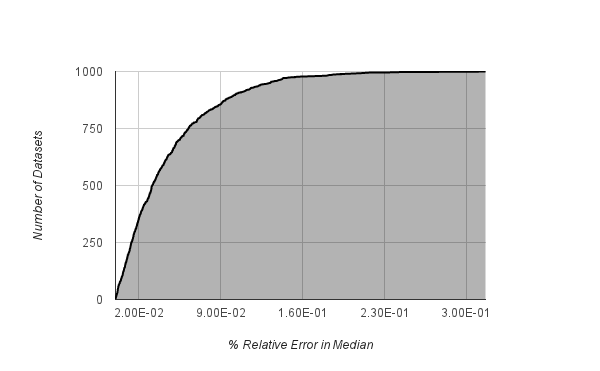
\includegraphics[scale=0.5]{img/relative_error}
\caption{CDF of Relative Error \label{fig:relative_error}}
\end{center}
\end{figure}

\subsection{Choosing the Number of Bins}
We did several experiments with the median container in order to figure out an optimum number of bins. The Number of bins affects the accuracy of the computed median. We used ten datasets generated randomly with different mean and variance. We used different number of bins ranging from 100 to 2000 for each dataset and calculated relative error in each case.

\begin{figure}[h]
\begin{center}
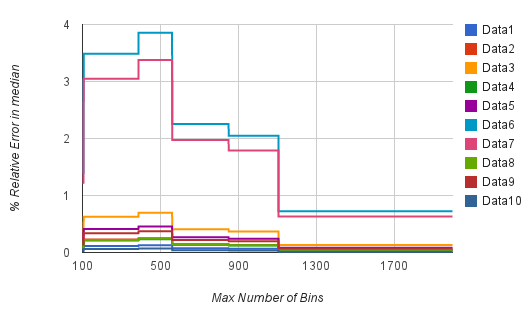
\includegraphics[scale=0.5]{img/bin_size_experiment}
\vspace*{-0.4cm}
\caption{\% Relative Error vs No of Bins \label{fig:binsize}}
\end{center}
\end{figure}

As evident from Figure \ref{fig:binsize}, bin size greater than 1200 gives the lowest error. We used bin size equal to 1200 while running Query 2.

\subsection{S Container}
We have to compute the number of plugs in a house having higher median load than the global median load (median load of all the plugs in the system). In order to efficiently compute this, we defined another container termed the $S$ container. The $S$ container stores median values of all the plugs in a house and evaluates the number of plugs higher than the global median. It provides basic operation of inserting (replacing) a newly computed plug median for the house, and finding out number of plugs which have higher median load than the global median (getNumOfLargeNum).

The issue here is, that we don't know number of plugs in a house before hand. It has to be acquired as the system makes progress. Hence, we had to use a map (key-value storage) in order to store the data but that leads to O(K) complexity of the \textit{getNumOfLargeNum} operation where K is the total number of plugs in a house. We avoided this by again using an array and stored all the data in sorted order with key being the plug median. When a new value is to be inserted, we require the old plug median in order to search the location of the plug data in the array. As soon as we find the location, we replace the new median with the old median and modify the location such that the array is sorted again.

The asymptotic complexity of this is also O(K) but in the given scenario, a momentous change in median values are unlikely. It will take finite number of more than one steps which will lead to significant change in the median values. In such a case, very little movement will be required while sorting the array after an insertion is performed. On the other hand, \textit{getNumOfLargeNum} operation will always be $\log(K)$.

%We do not store the whole measurement (16 byte) in the array but just the pointers (4 byte) to those measurements, which leads to even less amount of shift in the data. We use \textit{memmove} operation provided by CString library of C++, rather than manual copying of the array to increase the performance of the container.

%\subsection{Linked List Window}
 
\subsection{Experimental Evaluation}
We use the same setup as we used in case of Query 1. The broker process is executed on 1 Virtual Machine and Q2 process is execute on another virtual machine in the same cluster. We are able to achieve a constant average throughput of 480 thousand events per sec as shown in Figure \ref{fig:q2_throughput}

\begin{figure}[h]
\begin{center}
	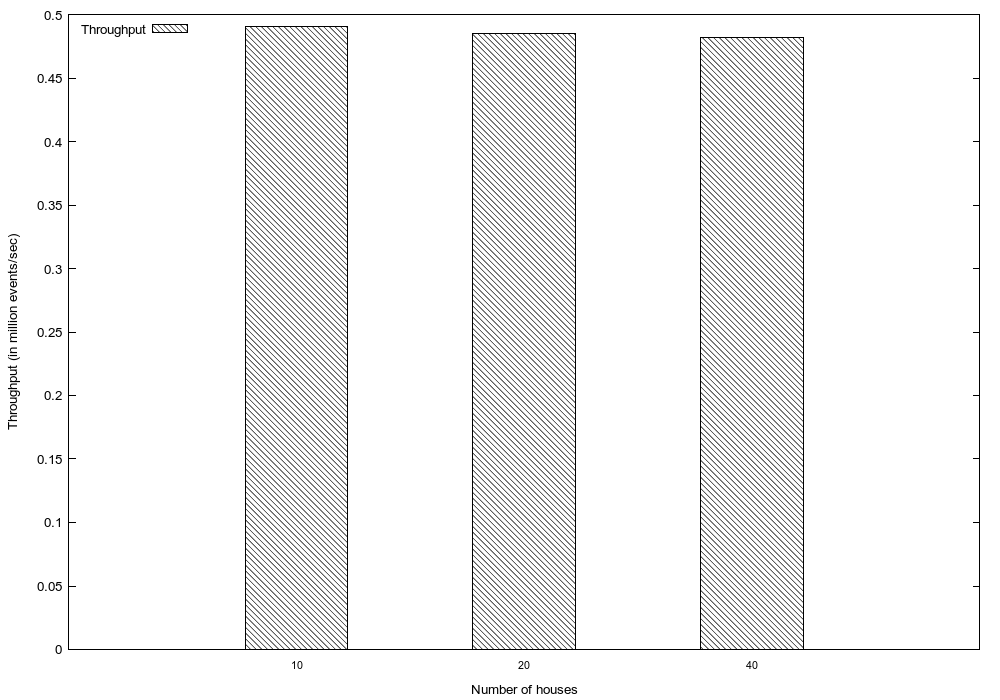
\includegraphics[scale=0.55]{img/q2_throughput}
	\vspace*{-0.4cm}
	\caption{Throughput vs No. of Houses (Query 2) \label{fig:q2_throughput}}
\end{center}
\end{figure}

\vspace*{-0.5cm}
Because there is only one Q2 process computing all the percentage values, throughput doesn't change significantly in terms of events/sec as the number of house increases. The utilization level in case of Q2 process is always close to 100\% as shown in Figure \ref{fig:q2_util}.

\begin{figure}[h]
\begin{center}
	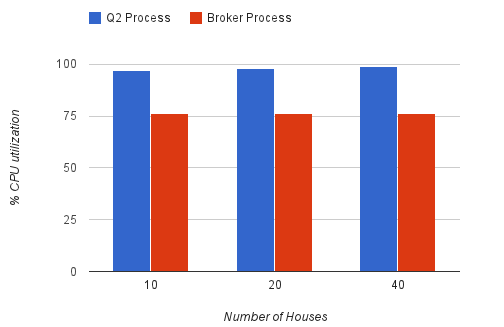
\includegraphics[scale=0.55]{img/q2_utilization}
	\vspace*{-0.3cm}
	\caption{\% Util vs No. of Houses (Query 2) \label{fig:q2_util}}
\end{center}
\end{figure}

\vspace*{-0.4cm}

\begin{figure}[h]
\begin{center}
	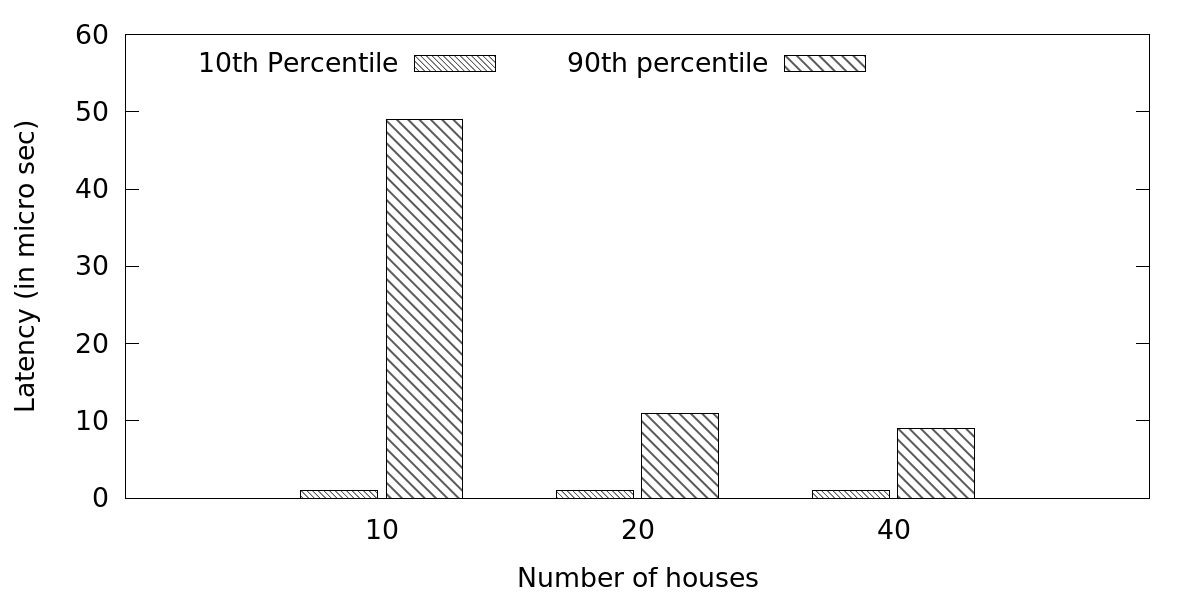
\includegraphics[scale=0.6]{img/q2_latency}
	\vspace*{-0.3cm}
	\caption{Latency vs No. of Houses (Query 2) \label{fig:q2_latency}}
\end{center}
\end{figure}

\vspace*{-0.4cm}
Latency corresponding to an output event, in case of Query 2, is defined as the amount of time taken to output event after the corresponding input event is received. Note that one input event may result in more than one output events and latency of the events output later will be higher. Latency graph for Query 2 is shown in Figure \ref{fig:q2_latency}. 90\% for 10 houses is higher because of biased distribution of data with respect to house. Houses 0-9 have more amount of data and the number of output events, therefore, will be more for every input event. In such a case, the events output later will have higher latency values.


\section{Query 1}
Query 1 requires us to forecast the average load of each plug and each house in the system for different time windows of length 1 min, 5 min, 15 min, 60 min and 120 min. For example, there will be $(24*60/15) = 96$ slots in a day corresponding to the time slice of length 15 min; for the 60 min slice, there will be $(24*60/60) = 24$ slots in a day and so on. The average load forecast is computed over all possible slots of all the time slices.

In order to make a forecast, we use two values - current average load and median load for the slot of given time slice. Using these 2 values, we forecast the average load for the next to next slot of the same time slice. We put out a forecast every 30 sec i.e. for each time slice we compute average load whenever we accumulate more data for next 30 seconds.

\subsection{Architecture}
The system consists of a broker process and house processes per house. The broker reads the data file and creates an event stream for each house process as shown in the figure \ref{fig:sysarch1}. The House process is responsible to forecast the average load of the house and all plugs in the house.

\begin{figure}[h]
\begin{center}
\begin{tikzpicture}[scale=0.8, >=stealth', transform shape, shorten >=1pt, node distance=2cm,auto]
\tikzstyle{every state}=[draw=blue!50, very thick, fill=blue!20]
\node[state] (broker) [text width=1.2cm, align=center] {Broker Process};

\node[state] (h2) [right of=broker,text width=1.2cm, align=center, node distance=4cm] {House 2 Process};
\node[state] (h1) [above of=h2,,text width=1.2cm, align=center] {House 1 Process};
\node[state] (h3) [below of=h2,text width=1.2cm, align=center] {House 3 Process};

\path[->] (broker) edge node[midway, sloped, anchor=south] {h1 events} (h1);
\path[->] (broker) edge node[midway] {h2 events} (h2);
\path[->] (broker) edge node[midway, sloped, anchor=south] {h3 events} (h3);
\end{tikzpicture}
\caption{System Architecture (Query 1)}
\end{center}
\label{fig:sysarch1}
\end{figure}

In the house process, we keep a 30 second accumulator for each plug. Whenever we receive an event for a plug, we increment the accumulator with the load\footnote{For now, we are ignoring events with work values} value in the received event. We store a count of values we receive with the timestamp within last 30s in order to compute the average later. We also keep load value accumulators for different time slices (1m, 5m, 15m, 60m and 120m). 

As soon as we receive an event crossing the 30s time window, we compute the forecast for all time slices using the sum of the load in the accumulator and the number of events received. We reinitialize the 30s accumulator to the load value in the received event and count to 1. A forecast is made for all the current time slots, whose slot boundary is crossed i.e. the received event does not belong to the current slot. We predict the average load for the next to next slot for such time slices using the average load and the historical median of the corresponding slot. The accumulators and count for such time slices get reset to zero. We output the forecast as zero if all the data is missing in a slot for a time slice. Note that, the above algorithm is based on the assumption that the timestamp of events coming from the broker never decreases. We, therefore, can make the forecast whenever any event corresponding to any plug in the house, crossing the current time slot for a time slice is received.

We defined a Median Container (MC) to compute exact median in case of query 1. The MC provides an interface to insert a new element and retrieve the median of all the elements currently in the container. We insert the average load of a plug or house for a given slot of fixed time slice into the container as soon as we compute it. The container returns the exact median of all the average values inserted into it.

\subsection{Median Algorithm (MC)}
We have used an exact algorithm to compute median of average loads in case of Query 1. We store all the previous days average loads in the container for a given time slot of any time slice.

We maintain two heaps inside the container. One of the heap is a min heap and stores the higher half of the values inserted into the container. On the other hand, second heap is a max heap and stores the lower half, of the values. If the total number of values inserted, are odd, we keep the median value in a separate variable. Now the following cases are possible:
\begin{itemize}
\item If the total number of values are odd, the extra variable stores the median.
\item If the total number of values are even, the median would be average of the root of both the heaps.
\end{itemize}

\noindent When a new value is inserted into the container, following cases can occur:
\begin{itemize}
\item If the total number of elements are odd before insertion, first we find out the lower value between the inserted value and the extra element. We, then, insert the lower value to the max heap and the other value to the min heap.
\item If the total number of elements are even before insertion, we insert the value in either min or max heap such that the invariant that the max heap contains the lowest values and the min heap contains the highest values is maintained. We keep one extra element in a separate variable as explained earlier.
\end{itemize}

\noindent Asymptotic complexity of the above algorithm in number of input elements (N) is as follows-

\begin{table}[h]
\begin{center}
\begin{tabular}{|c|c|}
\hline 
& Asymptotic Complexity \\ 
\hline 
insert & O($\log N$) \\ 
\hline 
getMedian & O(1) \\ 
\hline 
\end{tabular}
\end{center}
\end{table}

\vspace*{-0.5cm}
\subsection{Prediction Model}
We have used Weighted Average with Adaptive Weights prediction model in order to forecast the average load of a house or a plug. The predicted average load for a given time slot of a given time slice is computed as follows-
\begin{align*}
\mbox{Predicted Load} &= \mbox{W}*\mbox{History Median} \\ &+ (1-\mbox{W})*\mbox{Current Average}
\end{align*}

\noindent Where \textit{History Median} is the median of average loads of previous days for the same time slot of same time slice and W is the weight that we are assigning to \textit{History Median} in comparison with \textit{Current Average}. We make the prediction for next to next time slot of same time slice. Hence, \textit{Current Average} is the average of last to last time slot. We give equal weights to \textit{History Median} and \textit{Current Average} in the beginning and set the initial value of the weight \textit{W} as 0.5. As the program execution progresses, the value of \textit{W} is adapted based on the actual value we receive for each output forecast. We define the error in the forecast as follows-
\begin{align*}
\mbox{Error} &= (\mbox{Actual Load} - \mbox{Predicted Load})^2\\ &+ \lambda * (\mbox{W}_{new} - \mbox{W})^2
\end{align*}

\noindent $\lambda$ is a parameter to control the learning over W. \textit{Predicted Load} is computed using $\mbox{W}_{new}$.  Our goal is to minimize the above Error. We differentiate the Error with respect to $\mbox{W}_{new}$ and get the following expression when equated to 0-
\begin{align*}
\mbox{W}_{new} &= \frac{\mbox{W}*\lambda-(\mbox{AL}-\mbox{CA}) * (\mbox{HM}-\mbox{CA})}{\lambda + (\mbox{HM}-\mbox{CA})^2}
\end{align*}

\noindent Where AL=Actual Load, CA=Current Average, HM = History Median. Note that we use different weights for different houses for each time slice. We tried different values of $\lambda=0.01, 2, 100$ and we achieved minimum error in case of $\lambda = 2$. $\lambda$ is fixed throughout the experiment.

\subsection{Experimental Evaluation}
We executed our solution on a cluster of KVM \cite{kvm}  Virtual Machines. The broker runs on a single core 2.1GHz virtual machine, with 1 GB memory attached to a 10 Gbit local area network running Ubuntu 12.04. The Virtual Machine is running on Dual processor Intel Xeon E5 2620 base system. The house processes also run on a similarly configured Virtual Machines. We have done experiments running house processes on 1,2 and 4 Virtual Machines dividing the number of house processes equally amongst the VMs.

For throughput calculations, we redirected the output to the null file. Throughput will simply be the total number of input events divided by the total time taken in processing all the events. We did each experiment three times and took the average of the three throughput values.
\begin{figure}[h]
\begin{center}
	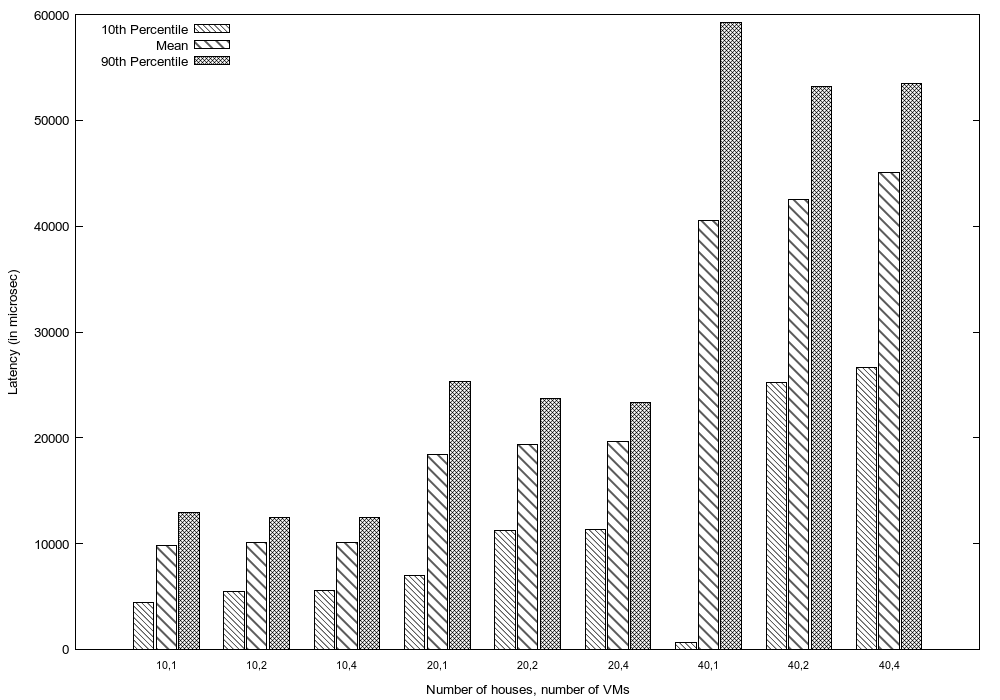
\includegraphics[scale=0.6]{img/q1_latency}
	\vspace*{-0.4cm}
	\caption{Latency vs No of Houses (Query 1) \label{fig:q1_latency}}
\end{center}
\end{figure}

\vspace*{-0.4cm}
As we increase the number of virtual machines, the latency values do not change much as shown in Figure \ref{fig:q1_latency}. because the broker becomes the bottleneck. The disk read in the broker limits the scalability of the system. On the other hand, throughput remains nearly constant in all the experiments as shown in Figure \ref{fig:q1_throughput}.

\begin{figure}[h]
\begin{center}
	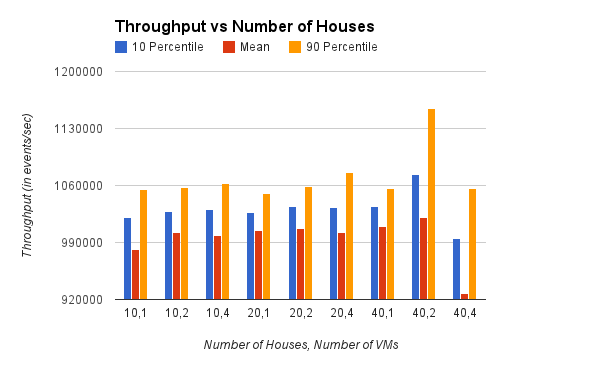
\includegraphics[scale=0.45]{img/q1_throughput}
	\vspace*{-0.4cm}
	\caption{Throughput vs No of Houses (Query 1)\label{fig:q1_throughput}}
\end{center}
\end{figure}

We contend based on utilization of CPU at the broker and house processes as evident from Figure \ref{fig:q1_util}, it is the broker that is currently limiting the scalability of the system.  The parsing of the read event accounts for most of the time spent by the broker on the CPU. If we were getting events as a stream and can avoid both the disk I/O and conversion of strings to numbers, we can witness the scalability of the system as a whole since the house processes are separate and can be run on different cores. 

\begin{figure}[h]
\begin{center}
	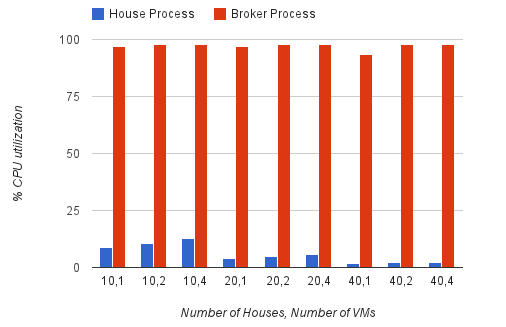
\includegraphics[scale=0.5]{img/q1_utilization}
	\vspace*{-0.4cm}
	\caption{\% Utilization vs No of Houses (Query 1)\label{fig:q1_util}}
\end{center}
\end{figure}


\section{Query 2}
The goal of query 2 is to identify outliers that consume significantly higher amount of energy compared with the average consumption computed globally. A plug is counted as an outlier if median load of the plug is more than the median load of all the plugs in the system for a given sliding window (1 hr or 24 hrs). We need to produce an output event when the percentage of such plugs in a house changes from the previous position of the sliding window. 

\subsection{Architecture}
To evaluate Query 2, we have to compute global median i.e. median of all the data of all the plugs in the system acquired in a given sliding window of length 1 hr and 24 hrs. We compare the global median with the local plug medians and figure out the outliers in the system. All of this computation needs to be done every time we receive a new event. The frequent comparison of locally computed data with global data enforces a single node solution for all the houses in case of Query 2.

There are two processes in the system residing on different nodes. The broker process reads data from a file and sends events to the Q2 process. Q2 keeps a linked list of all the events of last 24 hrs in the order they have been received. Whenever a new event is received by Q2, we slide the window such that some of the events from the tail of the linked list are removed and the new event is inserted at the head. Further, required plug medians and global median are recomputed and change in the number of outlier plugs is written to the output file (denoting an output event).

\begin{figure}[h]
\begin{center}
\begin{tikzpicture}[scale=0.7, >=stealth', transform shape, shorten >=1pt, node distance=4cm,auto]
\tikzstyle{every state}=[draw=blue!50, very thick, fill=blue!20,minimum size=2cm]
\node[state] (broker) [text width=1.5cm, align=center] {Broker Process};
\node[state] (Q2) [right of=broker] {Q2 Process};

\path[->] (broker) edge node {events} (Q2);
\end{tikzpicture}
\caption{System Architecture (Query 2)}
\end{center}
\end{figure}
\vspace*{-0.3cm}

We use the Sliding Median Container (SlidingMc) in order to compute various medians and S Container (SCont) for the purpose of finding the number of outliers in every house. Let's assume an event \textit{E} is received by the Q2 process from the broker process with timestamp \textit{$T_E$}. Let's also assume the window size to be \textit{W} seconds which can be either 1 hr or 24 hrs. \textit{$T_W$} is the minimum timestamp which exists in the window of length \textit{W} terminating with the event E as shown in the Figure \ref{fig:linked_list}.

\begin{figure}[h]
\begin{center}
\begin{tikzpicture}[scale=0.8, transform shape, shorten >=1pt, node distance=0.8cm,auto]
\tikzstyle{every state}=[draw=blue!50, rectangle, very thick, fill=blue!20]
\node[state] (I1) {$T_0$};
\node[state] (I2) [right of=I1] {};
\node[state] (I3) [right of=I2] {};
\node[state] (I4) [right of=I3] {$$};
\node[state] (I5) [right of=I4] {$T_W$};
\node[state] (I6) [right of=I5] {$$};
\node[state] (I7) [right of=I6] {$$};
\node[state] (I8) [right of=I7] {$$};
\node[state] (I9) [right of=I8] {$T_E$};

\draw [decorate,decoration={brace,amplitude=10pt,mirror,raise=10pt},yshift=0pt] (I5.center) -- (I9.center);
\node (text) at (5,-1) {Window W};
\end{tikzpicture}
\caption{Linked List in Q2 process \label{fig:linked_list}}
\end{center}
\end{figure}

Note that there may be multiple events with the timestamp $T_W$ in the window. In such a case, we choose the left most event with the same timestamp $T_W$ in the linked list. Also, if the data corresponding to the timestamp $\tau = (T_E - W +1)$ is missing, then $T_W$ will be the first timestamp bigger than $\tau$ for which event for any plug in the system is present. Now, the algorithm proceeds as follows. We shift the left end of the window one event, keeping the right end fixed. We delete the oldest event from the median container of the corresponding plug and the global median container. Now, we compute new median of the plug and insert the new median into the S container of the house. S container is, then, queried to find out whether the percentage of outliers for a given house has changed after the shift. We output an event if any of the percentage for any house has changed. On the other hand, if the global median doesn't change, we only check the percentage number of outliers for the house corresponding to the deleted event.

We stop when the leftmost event in the window has the timestamp $T_W$. In the last slide, before computing any medians, we also insert the newly received event $E$ into the global median container and the median container of the plug of the event E. Rest of the computation remains same. To avoid redundant storage of the data, we keep the linked list only for 24 hrs sliding window, and keep a pointer to the first event of the 1 hr window in the same linked list.


\subsection{Median Algorithm}
In query 2, we have to compute the median of large amounts of data frequently. A trade off exists between the computational complexity and accuracy of the median so derived. We define a container which provides the basic functionality of inserting a new element, deleting a given element and finally providing the approximate median for currently existing data in the container. We first insert all the elements into the container corresponding to the sliding window. Every time we slide by 1 sec, we perform at most 2 operations. We delete the oldest event if it exists and insert the latest event in the window. Every insert and/or delete operation is followed by computation of median. We, therefore, want to minimize the complexity of median calculation. We, now, propose an algorithm to compute median which takes constant time for every operation in the given scenario with very low relative error.

The basic idea is to construct a histogram of the data using fixed number of bins (M-1)\footnote{The Algorithm is inspired from discussions on \url{http://stackoverflow.com/questions/638030}} . The histogram is then queried to find median of the data. We sort the first M distinct values inserted into the container and use them in order to build up the (M-1) bins. Every $i^{th}$ inserted value corresponds to the starting of $i^{th}$ bin and every bin is associated with a frequency. Frequency denotes the frequency of the data greater than equal to $i^{th}$ lowest value (including) and less than $(i+1)^{th}$ lowest values (excluding) among M inserted value into the container. We also store the index of the bin containing the median after an insertion or deletion is performed, cumulative sum of the frequencies upto and including the bin in which median resides and the total number of values inserted into the container.

Every time a new value is inserted, the frequency of the corresponding bin is incremented. On the other hand, if a value is to be deleted, the frequency of the corresponding bin is decremented. At the time of insertion or deletion, we also modify the variable storing the index of the bin having the current median and accordingly the cumulative sum. The corresponding bin to insert/delete can be found in $\log(M)$ order complexity where (M-1) represents the number of bins. We handle below cases as follows-
\begin{itemize}
\item If frequency of a bin becomes significantly higher than some constant times the average bin frequency, we split the bin into two bins. Every new bin is given half of the frequency of the original bin. The range of values is also equally divided between 2 bins.
\item If frequency of a bin reaches to zero, we simply delete the bin.
\item If an inserted value is less than the lowest value or higher than the highest value present in the median container, we create another bin starting with the inserted value.
\item If number of bins are higher than the maximum allowed number of bins, we merge 2 bins. These 2 consecutive bins are chosen such that they have minimum total frequency than any other two consecutive bins. The frequency of the higher bin is added to the frequency of the lower bin and the higher bin is deleted.
\end{itemize}

We implemented median container using an array. Arrays provides the flexibility of binary search which is required to be done frequently in our case. We keep two empty memory slots on both sides of the array, which simplifies an insertion of a new bin in case of inserted value not being in the existing range of values. When a new bin is inserted/merged in the middle of the array, we shift the rest of the array to fill up the void.  We used low level operation \textit{memmove} provided by cstring library in C++, in order to speed up the shift operation.

In this case we need to compute the median every time we receive an event. So every insert or deletion or both will be followed by a call to the \textit{getMedian} function of the container.  We modify the variable storing the index to the bin having the current median, at the time of insert and delete only.

\begin{table}[h]
\begin{center}
\begin{tabular}{|c|c|c|}
\hline 
 & \textbf{Worst Case} & \textbf{Average Case} \\ 
\hline 
\textbf{insert} & O(M) & O($\log(M)$) \\
\hline 
\textbf{delete} & O(M) & O($\log(M)$) \\
\hline 
\textbf{getMedian} & O(1) & O(1) \\ 
\hline 
\end{tabular} 
\end{center}
\end{table}

\subsection{Relative Error for Median Container}
In this case, we did 1000 experiments, each inserting 50000 random values into the container. The CDF is plotted in the Figure \ref{fig:relative_error}. It can be observed that there is very low relative error due to the approximation. 

\begin{figure}[h]
\begin{center}
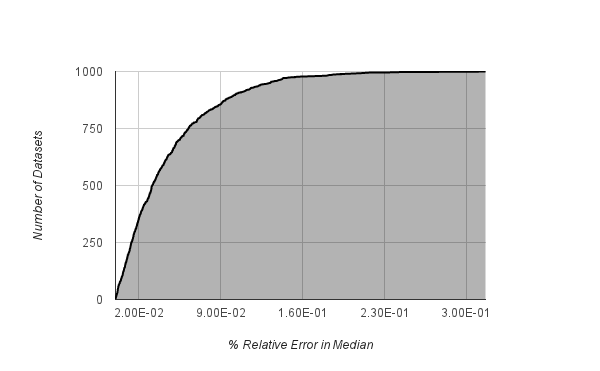
\includegraphics[scale=0.5]{img/relative_error}
\caption{CDF of Relative Error \label{fig:relative_error}}
\end{center}
\end{figure}

\subsection{Choosing the Number of Bins}
We did several experiments with the median container in order to figure out an optimum number of bins. The Number of bins affects the accuracy of the computed median. We used ten datasets generated randomly with different mean and variance. We used different number of bins ranging from 100 to 2000 for each dataset and calculated relative error in each case.

\begin{figure}[h]
\begin{center}
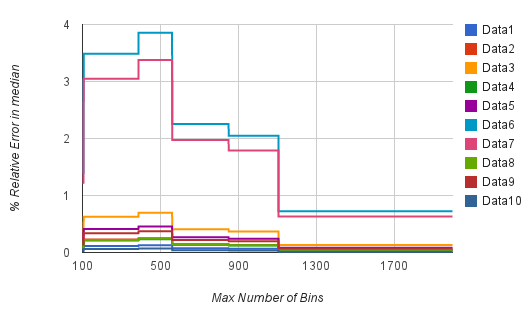
\includegraphics[scale=0.5]{img/bin_size_experiment}
\vspace*{-0.4cm}
\caption{\% Relative Error vs No of Bins \label{fig:binsize}}
\end{center}
\end{figure}

As evident from Figure \ref{fig:binsize}, bin size greater than 1200 gives the lowest error. We used bin size equal to 1200 while running Query 2.

\subsection{S Container}
We have to compute the number of plugs in a house having higher median load than the global median load (median load of all the plugs in the system). In order to efficiently compute this, we defined another container termed the $S$ container. The $S$ container stores median values of all the plugs in a house and evaluates the number of plugs higher than the global median. It provides basic operation of inserting (replacing) a newly computed plug median for the house, and finding out number of plugs which have higher median load than the global median (getNumOfLargeNum).

The issue here is, that we don't know number of plugs in a house before hand. It has to be acquired as the system makes progress. Hence, we had to use a map (key-value storage) in order to store the data but that leads to O(K) complexity of the \textit{getNumOfLargeNum} operation where K is the total number of plugs in a house. We avoided this by again using an array and stored all the data in sorted order with key being the plug median. When a new value is to be inserted, we require the old plug median in order to search the location of the plug data in the array. As soon as we find the location, we replace the new median with the old median and modify the location such that the array is sorted again.

The asymptotic complexity of this is also O(K) but in the given scenario, a momentous change in median values are unlikely. It will take finite number of more than one steps which will lead to significant change in the median values. In such a case, very little movement will be required while sorting the array after an insertion is performed. On the other hand, \textit{getNumOfLargeNum} operation will always be $\log(K)$.

%We do not store the whole measurement (16 byte) in the array but just the pointers (4 byte) to those measurements, which leads to even less amount of shift in the data. We use \textit{memmove} operation provided by CString library of C++, rather than manual copying of the array to increase the performance of the container.

%\subsection{Linked List Window}
 
\subsection{Experimental Evaluation}
We use the same setup as we used in case of Query 1. The broker process is executed on 1 Virtual Machine and Q2 process is execute on another virtual machine in the same cluster. We are able to achieve a constant average throughput of 480 thousand events per sec as shown in Figure \ref{fig:q2_throughput}

\begin{figure}[h]
\begin{center}
	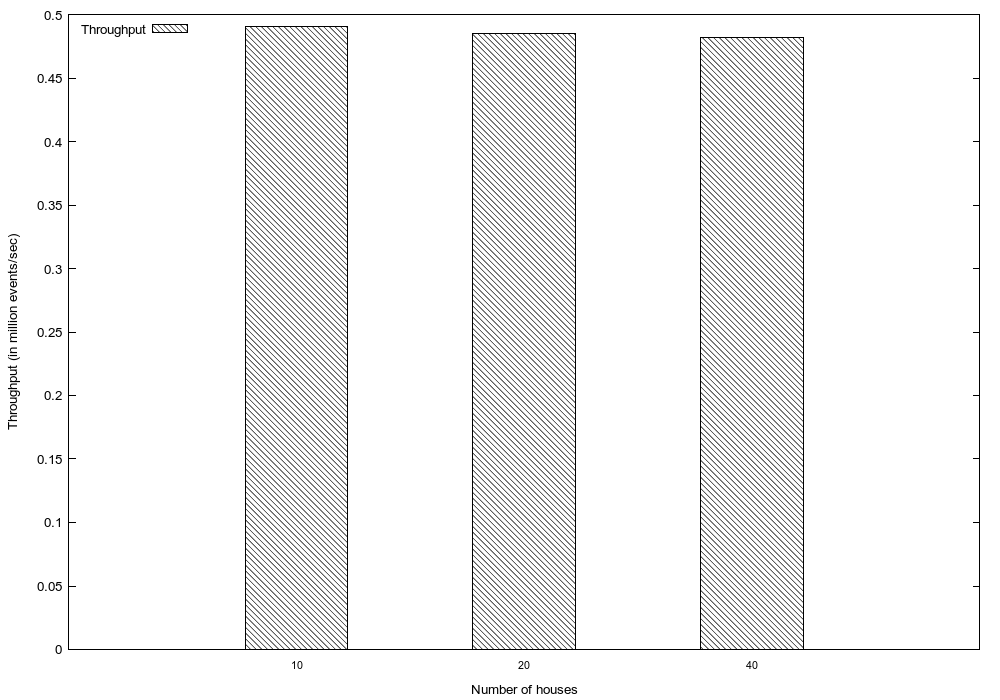
\includegraphics[scale=0.55]{img/q2_throughput}
	\vspace*{-0.4cm}
	\caption{Throughput vs No. of Houses (Query 2) \label{fig:q2_throughput}}
\end{center}
\end{figure}

\vspace*{-0.5cm}
Because there is only one Q2 process computing all the percentage values, throughput doesn't change significantly in terms of events/sec as the number of house increases. The utilization level in case of Q2 process is always close to 100\% as shown in Figure \ref{fig:q2_util}.

\begin{figure}[h]
\begin{center}
	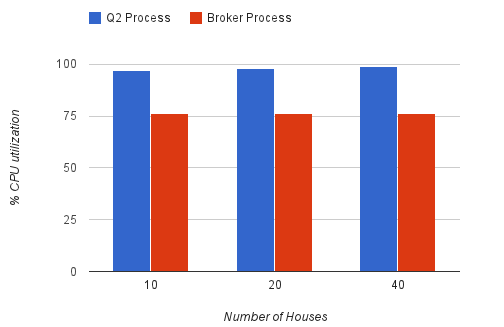
\includegraphics[scale=0.55]{img/q2_utilization}
	\vspace*{-0.3cm}
	\caption{\% Util vs No. of Houses (Query 2) \label{fig:q2_util}}
\end{center}
\end{figure}

\vspace*{-0.4cm}

\begin{figure}[h]
\begin{center}
	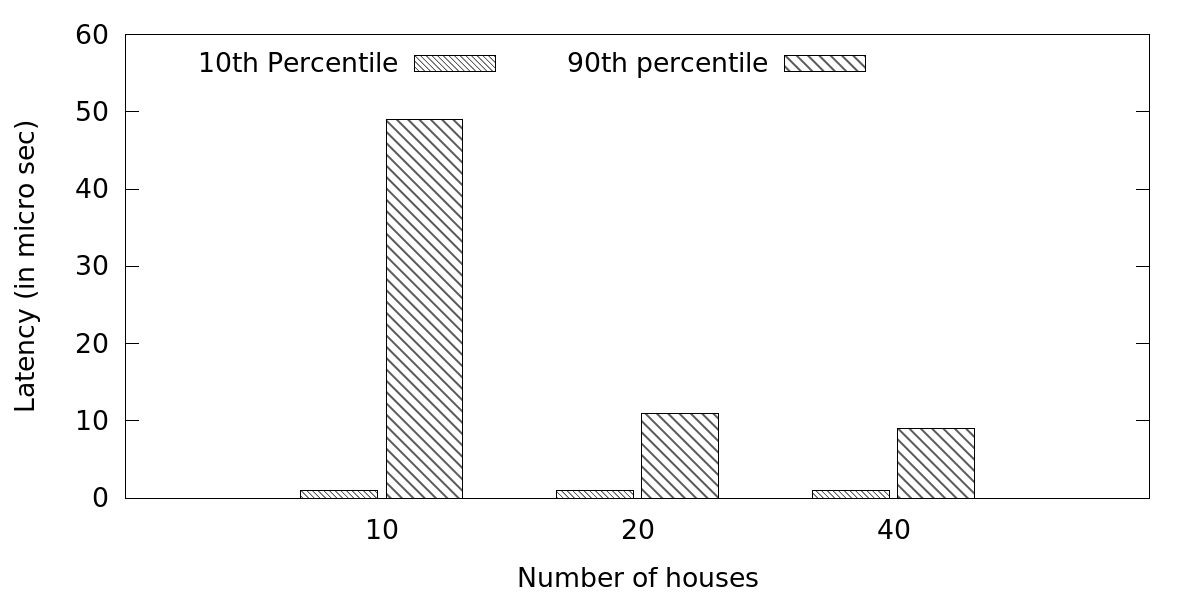
\includegraphics[scale=0.6]{img/q2_latency}
	\vspace*{-0.3cm}
	\caption{Latency vs No. of Houses (Query 2) \label{fig:q2_latency}}
\end{center}
\end{figure}

\vspace*{-0.4cm}
Latency corresponding to an output event, in case of Query 2, is defined as the amount of time taken to output event after the corresponding input event is received. Note that one input event may result in more than one output events and latency of the events output later will be higher. Latency graph for Query 2 is shown in Figure \ref{fig:q2_latency}. 90\% for 10 houses is higher because of biased distribution of data with respect to house. Houses 0-9 have more amount of data and the number of output events, therefore, will be more for every input event. In such a case, the events output later will have higher latency values.

\section{Future Work}
The presented solution does not use work values. We could use work values in case of Query 1 in order to compute total load for a given time window. We would only use work values for the average load computation of longer time slices such as \{60 min, 120 min\}. This would lead to more precise computation of average load for the time slot of a time slice.


\section{Conclusions}
%This file will contain conclusions

In summary, the main contributions of this work are:
1) A custom design and implementation of a smart grid plug load predictor and outlier identifier system.
It is our belief that the custom design led to the significant throughput we observed with the given data set.
In fact, the throughput of the system is much higher than what is reported because of the limitations of the broker process which is really not part of the predictor system.
2) A scalable architecture to process dense smart plug load data streams.
Every house process can be given it's own core to run on and so the scalability is limited to the number of house processes we want to process data for.
3) A fast and lightweight C++ implementation of the median based prediction heuristic for predicting the load at smart plugs for different time windows.
4) A method and code for efficiently sliding two different timeslice windows over a continuous stream of events.

While generic CEP engines such as Esper and Padres can also be used for this, it is our belief that the problem stated is really not a problem meant for CEP engines and hence our approach would work better than if we did employ such middleware.


%ACKNOWLEDGMENTS are optional
%\section{Acknowledgments}
%
% The following two commands are all you need in the
% initial runs of your .tex file to
% produce the bibliography for the citations in your paper.
\bibliographystyle{abbrv}
\bibliography{references}  % sigproc.bib is the name of the Bibliography in this case
% You must have a proper ".bib" file
%  and remember to run:
% latex bibtex latex latex
% to resolve all references
%
% ACM needs 'a single self-contained file'!
%
%APPENDICES are optional
%\balancecolumns

\end{document}
